\documentclass{article}

\usepackage[utf8]{inputenc}
\usepackage{graphicx}

\author{Navarro Presas Moisés Alejandro - 215861509}
\title{
RSA\\
Seminario de Solución de Problemas de Métodos Matemáticos I
}
\pagenumbering{gobble}

\begin{document}
  \maketitle
  \tableofcontents
  \newpage

  \section{RSA}
  RSA es un sistema criptografico de clave publica, es decir que utiliza enriptación asimetrica. En la actualidad es el sistema de encriptación mas utilizado por su robustes; ya que para logar romperlo, con computadoras normales, el proceso puede llevar años

  \subsection{Algoritmo}
  \emph{Obtención de llaves}\\
  \begin{enumerate}
    \item Se eligen dos numeros primos distintos $p$ y $q$
    \item Se calcula $n = pq$
    \item Se calcula $\varphi(n) = (p-1)(q - 1)$
    \item Se elige un numero positivo $e$ menor que $\varphi(n)$ y coprimo de $\varphi(n)$
    \item Se determina $d$ tal que  $d \cdot e \equiv 1 \pmod{\varphi(n)}$
  \end{enumerate}
  La llave publica $=(n, e)$\\
  La llave privada $=(n, d)$\\
  \\
  \emph{Cifrado}\\
  $c \equiv m^e \pmod{n}$\\
  \\
  \emph{Descifrado}\\
  $c \equiv m^d \pmod{n}$\\

  \section{Programa}
  El programa está desarrollado en python, y a su vez está dividido en tres archivos:
  \begin{enumerate}
    \item Generación de llaves (\emph{keygen.py})
    \item Encriptación (\emph{cipher.py})
    \item Desencriptación (\emph{decipher.py})
  \end{enumerate}

  \subsubsection{keygen.py}
  Lo primero que debemos hacer es obtener una lista con $n$ numeros primos, esto lo hacemos mediante la criba de Eratóstenes\\
  \begin{center}
    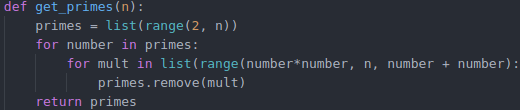
\includegraphics{img/get_primes.png}
  \end{center}
  Lo que se hace en este algoritmo es recorrer una lista de numeros (del 2 hasta el máximo deseado) e ir descartando todfos aquellos que son multiplos de un numero ya evaluado.\\
  \\
  De esta lista de numeros primos se eligen $p$ y $q$\\
  \begin{center}
    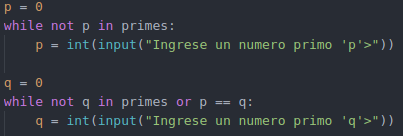
\includegraphics{img/get_p_q.png}
  \end{center}

  Posteriormente se calcula tanto $n$ como $\varphi(n)$\\
  \begin{center}
    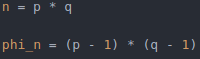
\includegraphics{img/calculate_n_phin.png}
  \end{center}

  Despues se generan las posibles llaves publicas
  \begin{center}
    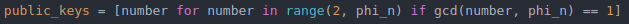
\includegraphics{img/public_keys.png}
  \end{center}
  Esto se lográ revisando todos los numeros entre 2 y $\varphi(n)$, tomando aquellos cuyo $gcd$ con respecto de $\varphi(n)$ sea igual a 1\\
  \\
  Se selecciona una de estas posible llaves publicas ($e$)
  \begin{center}
    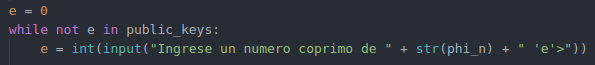
\includegraphics{img/get_e.png}
  \end{center}

  Finalmente se calcula el inverso multiplciativo de $e \pmod{n}$
  \begin{center}
    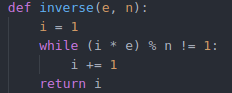
\includegraphics{img/inverse.png}
  \end{center}

  \subsubsection{cipher.py}
  El proceso de cifrado es bastante simple, tan solo hay que elevar el dato a cifrar ($c$) a la potencia $e$ y posteriormente obenter su modulo $n$
  \begin{center}
    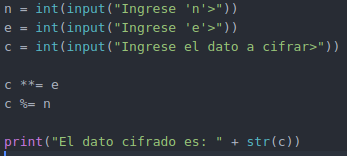
\includegraphics{img/cipher.png}
  \end{center}

  \subsubsection{decipher.py}
  El proceso de para descifrar es simialar al de cifrado, tan solo hay que elevar el dato a cifrar ($c$) a la potencia $d$ y posteriormente obenter su modulo $n$
  \begin{center}
    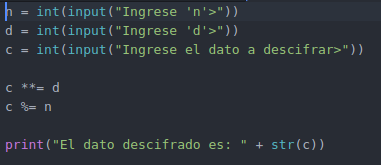
\includegraphics{img/decipher.png}
  \end{center}





\end{document}
